\documentclass[11pt]{article}
\usepackage[margin=1in]{geometry}
\usepackage{listings}
\usepackage{xcolor}
\usepackage{graphicx}
\usepackage{enumitem}

\lstset{
  basicstyle=\ttfamily\footnotesize,
  commentstyle=\color{gray},
  language=C++,
  breaklines=true,
  showstringspaces=false
}

\setlength{\parindent}{0pt}
\setlength{\parskip}{8pt}

\begin{document}

Karishma Premnath \\
EECE 7205, Stacks and Queues, In-Class Work \\
Q1 Expression Evaluation Using Stacks

\hrulefill

\textbf{(a) Functions}

\begin{itemize}[leftmargin=*, itemsep=2pt, topsep=2pt]
\item \texttt{isNumber(t)} \quad a token is a number if it is all digits, or a minus sign
      followed by digits. This is how \texttt{-7} is read as a value and not as subtraction.
\item \texttt{precedence(op)} \quad \texttt{\^{}} is 3, \texttt{*} and \texttt{/} are 2,
      \texttt{+} and \texttt{-} are 1.
\item \texttt{applyOp(a, b, op)} \quad does one operation on two integers,
      with \texttt{a} as the left operand. Division calls \texttt{floorDiv}.
\item \texttt{floorDiv(a, b)} \quad rounds down toward negative infinity by subtracting one
      when the signs differ and the division is not exact.
\item \texttt{evaluate(tokens)} \quad pushes numbers on the values stack, and before pushing
      an operator it applies every waiting operator that must go first.
\item \texttt{IntStack} and \texttt{CharStack} \quad the two stacks, one holding
      \texttt{int} values and one holding \texttt{char} operators.
\end{itemize}

The pop rule inside \texttt{evaluate}:

\begin{tabular}{ll}
Top of operators stack is & Then \\[2pt]
\hline
higher precedence & apply it before pushing \\
equal precedence, new operator is \texttt{+ - * /} & apply it (left associative) \\
equal precedence, new operator is \texttt{\^{}} & leave it (right associative) \\
lower precedence & leave it \\
\end{tabular}

\textbf{(b) Evaluate $8 + 3 * 2 \wedge 2 - 20 / 4$}

\begin{tabular}{llll}
Step & Operator & Calculation & Expression left \\[2pt]
\hline
    &            &                 & \texttt{8 + 3 * 2 \^{} 2 - 20 / 4} \\
1 & \texttt{\^{}} & $2 \wedge 2 = 4$   & \texttt{8 + 3 * 4 - 20 / 4} \\
2 & \texttt{*}    & $3 \times 4 = 12$  & \texttt{8 + 12 - 20 / 4} \\
3 & \texttt{/}    & $20 / 4 = 5$       & \texttt{8 + 12 - 5} \\
4 & \texttt{+}    & $8 + 12 = 20$      & \texttt{20 - 5} \\
5 & \texttt{-}    & $20 - 5 = 15$      & \texttt{15} \\
\end{tabular}

Step 1 goes first because \texttt{\^{}} has the highest precedence. Steps 2 and 3 come next
and are taken left to right, then steps 4 and 5 the same way.

\textbf{Answer: 15}

\textbf{(c) Trace}

The two stacks after each token is processed:

\begin{tabular}{llll}
Token & Action & Values (bottom to top) & Operators \\[2pt]
\hline
\texttt{8}  & push 8 & 8 & \\
\texttt{+}  & push \texttt{+} & 8 & \texttt{+} \\
\texttt{3}  & push 3 & 8 3 & \texttt{+} \\
\texttt{*}  & push \texttt{*} & 8 3 & \texttt{+ *} \\
\texttt{2}  & push 2 & 8 3 2 & \texttt{+ *} \\
\texttt{\^{}}  & push \texttt{\^{}} & 8 3 2 & \texttt{+ * \^{}} \\
\texttt{2}  & push 2 & 8 3 2 2 & \texttt{+ * \^{}} \\
\texttt{-}  & apply \texttt{\^{}}, \texttt{*}, \texttt{+}, then push \texttt{-} & 20 & \texttt{-} \\
\texttt{20} & push 20 & 20 20 & \texttt{-} \\
\texttt{/}  & push \texttt{/} & 20 20 & \texttt{- /} \\
\texttt{4}  & push 4 & 20 20 4 & \texttt{- /} \\
\end{tabular}

At token \texttt{-}, three operators are applied because \texttt{-} is weaker than all three
waiting on the stack:

\begin{tabular}{lll}
Apply & Calculation & Values after \\[2pt]
\hline
\texttt{\^{}} & $2 \wedge 2 = 4$ & 8 3 4 \\
\texttt{*}    & $3 \times 4 = 12$ & 8 12 \\
\texttt{+}    & $8 + 12 = 20$ & 20 \\
\end{tabular}

Remaining calculations once the tokens are finished:

\begin{tabular}{lll}
Apply & Calculation & Values after \\[2pt]
\hline
\texttt{/} & $20 / 4 = 5$ & 20 5 \\
\texttt{-} & $20 - 5 = 15$ & 15 \\
\end{tabular}

\textbf{Result: 15}

\textbf{(d) Tests}

\begin{tabular}{lll}
Expression & Answer & Wrong answer if mishandled \\[2pt]
\hline
\texttt{2 \^{} 3 \^{} 2} & 512 & 64 \\
\texttt{-7 / 2} & $-4$ & $-3$ \\
\end{tabular}

$2 \wedge 3 \wedge 2$ gives \textbf{512}. When the second \texttt{\^{}} arrives, the first one has
equal precedence, and \texttt{\^{}} is right associative, so it is left waiting instead of being
applied. That makes $3 \wedge 2 = 9$ run first, then $2 \wedge 9 = 512$. Treating \texttt{\^{}} as
left associative would give $(2 \wedge 3) \wedge 2 = 64$.

$-7 / 2$ gives \textbf{-4}. The exact value is $-3.5$. C++ integer division cuts the fraction
off toward zero and gives $-3$, but the question asks for rounding down toward negative
infinity, which is $-4$. \texttt{floorDiv} subtracts one because the signs differ and the
division is not exact. A clean division such as $-20 / 4$ is untouched and stays $-5$.

\newpage
\textbf{Code}

\lstinputlisting{expression_eval_short.cpp}

\textbf{Output}

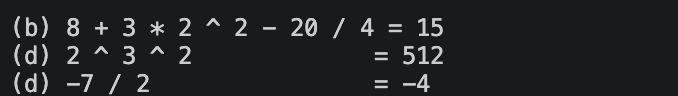
\includegraphics[width=\linewidth]{output_screenshot.png}

\end{document}
